\section{Output}
\subsection{Files}

Explain the created C++ files and executables, and how to use them.

\subsection{Two-scale algorithm}

Explain the structure of the two-scale algorithm classes and how they
work and are plugged together.

\begin{figure}[tb]
  \centering
  \tikzumlset{fill class=white}
  \begin{tikzpicture}
    \umlclass[x=0, y=0, type=abstract]{Beta\_function}{}{
      + \umlvirt{display() : const Eigen::ArrayXd} \\
      + \umlvirt{set(v : const Eigen::ArrayXd\&) : void}\\
      + \umlvirt{beta() : Eigen::ArrayXd}
    }
    \umlclass[x=8, y=0, type=abstract]{Two\_scale\_model}{}{
      + \umlvirt{calculate\_spectrum() : void}\\
      + \umlvirt{run\_to(scale : double, eps : double) : int}\\
      + \umlvirt{set\_precision(precision : double) : void}
    }
    \umlclass[x=0, y=-4]{MSSM\_susy\_parameters}{}{
      + display() : const Eigen::ArrayXd \\
      + set(v : const Eigen::ArrayXd\&) : void\\
      + beta() : Eigen::ArrayXd
    }
    \umlclass[x=0, y=-8]{MSSM\_soft\_parameters}{}{
      + display() : const Eigen::ArrayXd \\
      + set(v : const Eigen::ArrayXd\&) : void\\
      + beta() : Eigen::ArrayXd
    }
    \umlclass[x=0, y=-12]{MSSM$<$Two\_scale$>$}{}{
      + calculate\_spectrum() : void\\
      + run\_to(scale : double, eps : double) : int\\
      + set\_precision(precision : double) : void
    }
   \umlinherit{MSSM\_susy\_parameters}{Beta\_function}
   \umlinherit{MSSM\_soft\_parameters}{MSSM\_susy\_parameters}
   \umlinherit{MSSM$<$Two\_scale$>$}{MSSM\_soft\_parameters}
   \umlinherit[geometry=-|]{MSSM$<$Two\_scale$>$}{Two\_scale\_model}
  \end{tikzpicture}
  \caption{Two-scale model class hierarchy}
  \label{fig:two-scale-class-hierarchy}
\end{figure}

\subsection{Lattice algorithm}

Explain the structure of the lattice algorithm classes and how they
work.
